\section{Architecture}\label{sec:architecture}

The Åboat already has an architecture of its own. The system is already functional (though it has its own communication protocol). What we aim to do is build on top of this architecture.
\\\\
Currently, the Åboat has an architecture that consists of microservices. Each of these microservices runs a different “functionality” of the boat. There are microservices for sensors, control, storage, and communication. The current picture of the Åboat architecture can be seen in the image below.

\begin{figure}[ht]
	\centering
	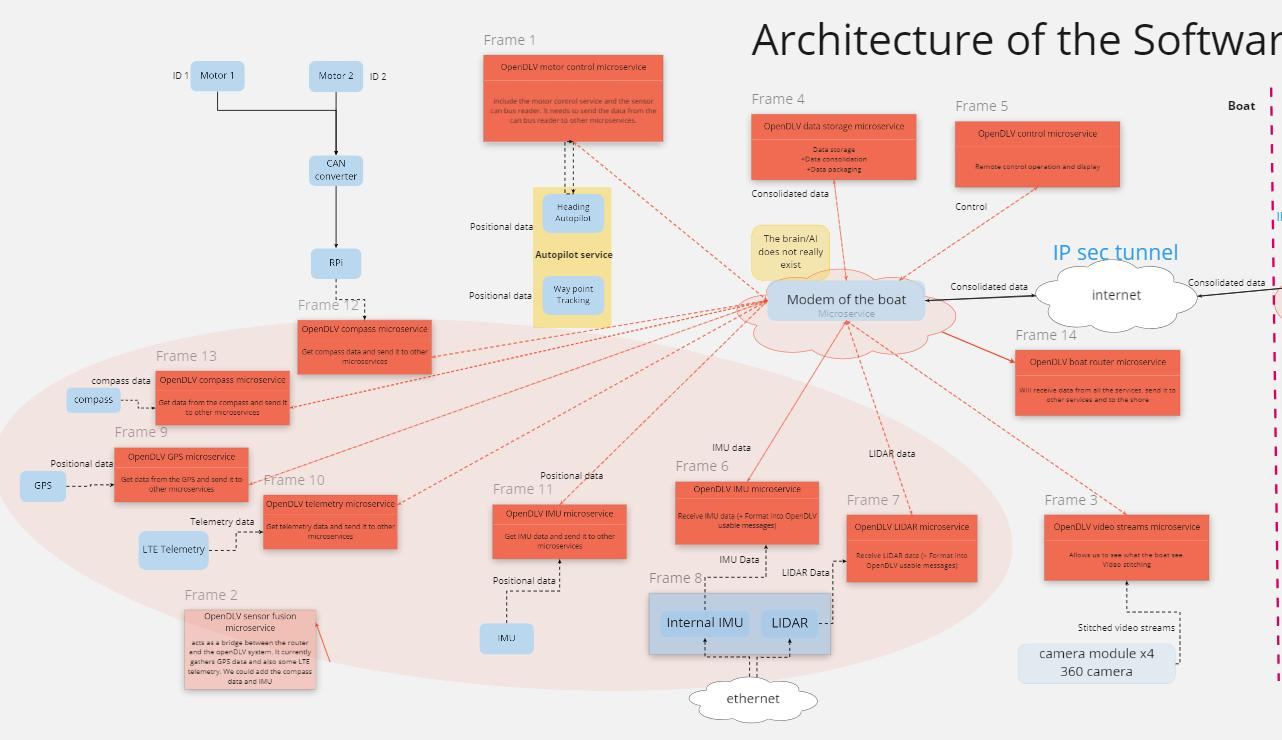
\includegraphics[width=\linewidth]{images/aboat-architecture}
	\caption{Åboat architecture}
	\label{fig:aboat-architecture}
\end{figure}

The purpose of the VRGP implementation is to create an independent system implementing the VRGP specification, which will interface with the existing architecture of the Åboat. The interfacing will be achieved through a microservice (called an \textbf{adapter}), which has the sole purpose of translating the calls between the Åboat and the VRGP service. This will make the VRGP service completely independent of the vessel that uses it, thus achieving a good level of decoupling.
\\\\
Using the VRGP service with other boats would then be easy, as the only component that would have to be rewritten would be the \textbf{adapter}, which, as mentioned above, is only a small layer that interfaces between the vessel and VRGP service.
\\\\
On the shore-side, there is the MOC service, which consists of a backend and potentially multiple frontends attached to it. The backend is responsible for the communication with the vessel-side (more specifically, the VRGP service), while the frontend is responsible for displaying the information to (most likely) human operators.
\\\\
An image of the current architecture of the VRGP implementation can be seen below.

\begin{figure}[ht]
	\centering
	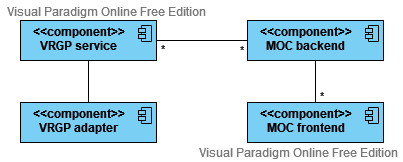
\includegraphics[width=\linewidth]{images/vrgp-architecture}
	\caption{VRGP architecture}
	\label{fig:vrgp-architecture}
\end{figure}

More details about the components are presented in the implementation section below (section \ref{sec:technologies}).

\section{Design}\label{sec:design}

In the following sections, we describe our current design using several UML diagrams. UML is used for most parts of the design for now, as it provides a well-known, easy to understand and somewhat unambiguous description of the design. Some of the diagrams present the high-level views of the system, while others are more in-depth.

\subsection{Static Design}

\subsubsection{Deployment Diagram}

The deployment diagram provides an overview of the different deliverables for this software project and in which environments they can be used. The most important artifact to be delivered is the VRGP service (which is the actual VRGP implementation), while the other deliverables (the OpenDLV adapter, the MOC backend and frontend) are mostly built around the service and aim to show that it works. The deployment diagram is shown in figure \ref{fig:deployment-diagram}.

\begin{figure}[ht]
	\centering
	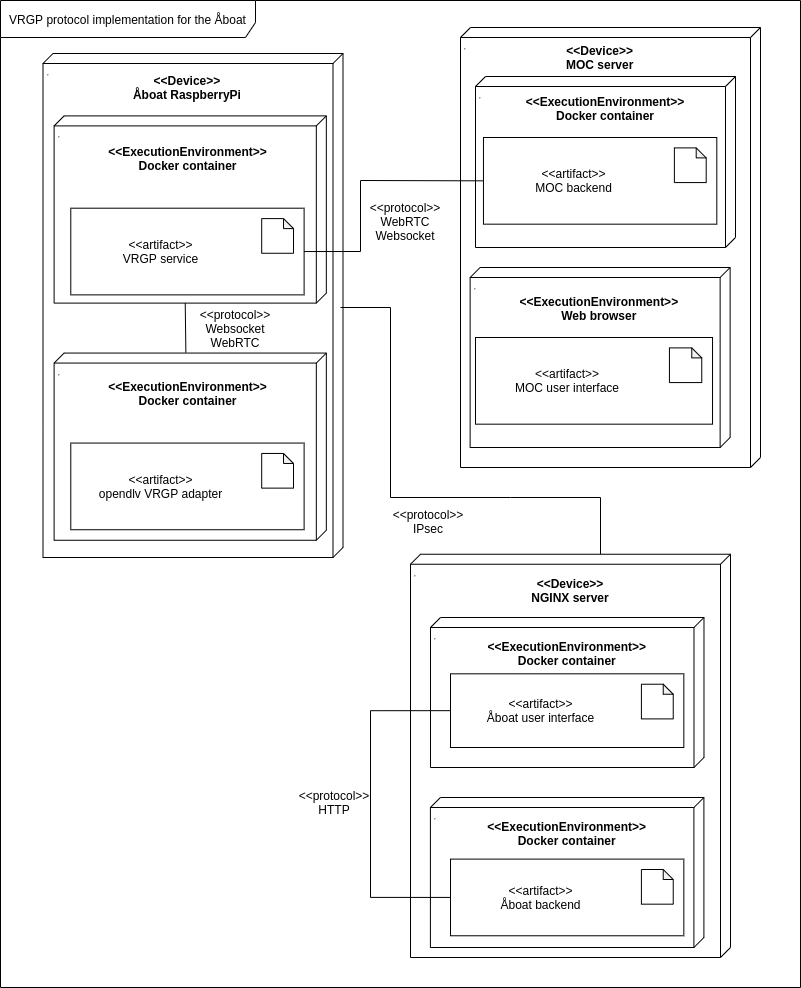
\includegraphics[width=\linewidth]{diagrams/deployment-diagram}
	\caption{Deployment diagram}
	\label{fig:deployment-diagram}
\end{figure}

\subsubsection{Component Diagrams}

The high-level components have been briefly described in the introduction above.
\\\\
The most important part of the communication happens between the vessel-side and the shore-side, i.e. between the VRGP service and the MOC. A diagram illustrating this connection can be seen in figure \ref{fig:vrgp-moc-component-diagram}.
\\\\
As can be seen, the component diagram mostly follows the requirements outlined above (\ref{sec:func-requirements}).
\\\\
Another important part of the communication happens between the VRGP service and the adapter microservice. The communication can be seen in figure \ref{fig:adapter-vrgp-component-diagram}.
\\\\
The left side depicts the OpenDLV microservice running the adapter, which will have further communications with the other Åboat microservices.

\begin{landscape}

\begin{figure}[!p]
	\centering
	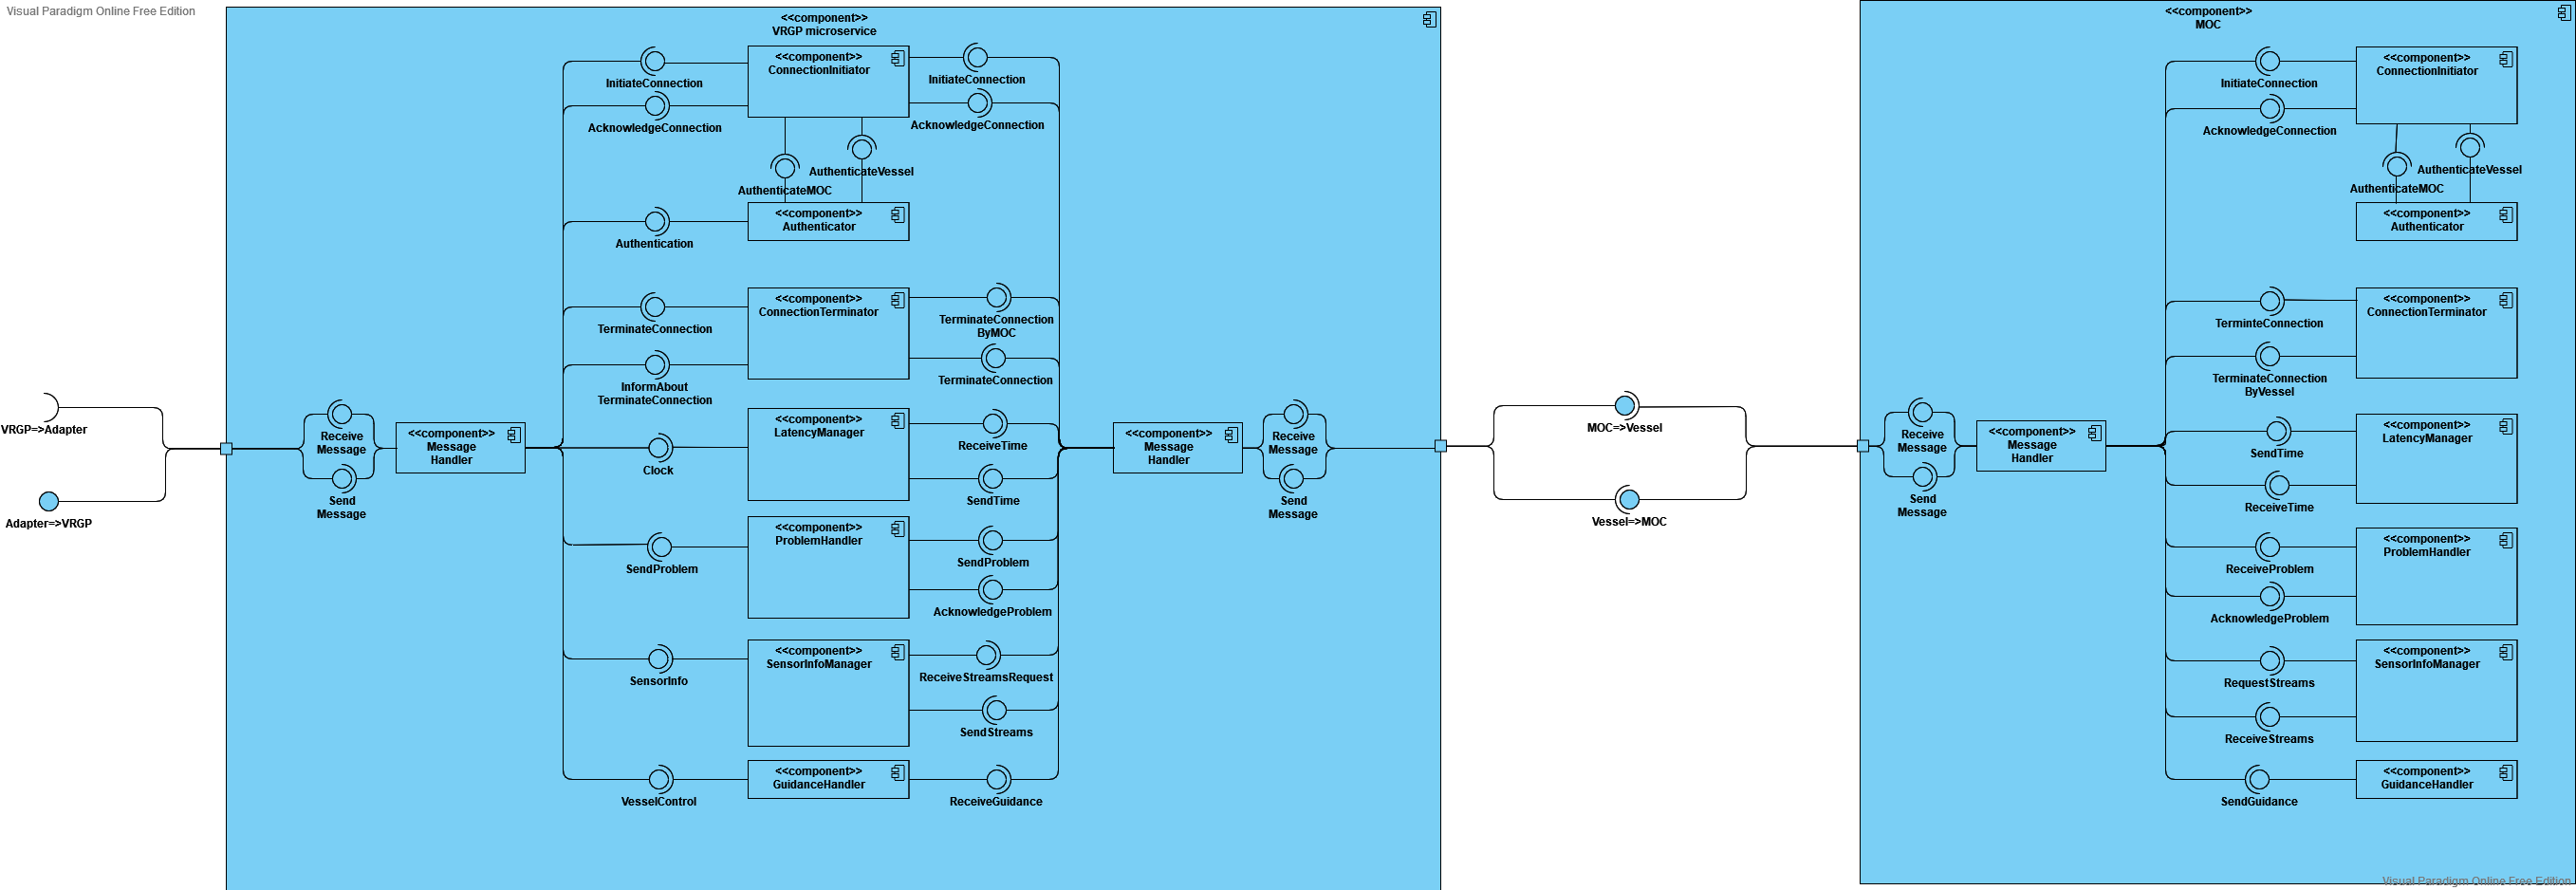
\includegraphics[width=\linewidth]{diagrams/ComponentDiagram_GenericVrgpMicroservice_HandlerView}
	\caption{VRGP service - MOC component diagram}
	\label{fig:vrgp-moc-component-diagram}
\end{figure}

\end{landscape}

\begin{landscape}

\begin{figure}[!p]
	\centering
	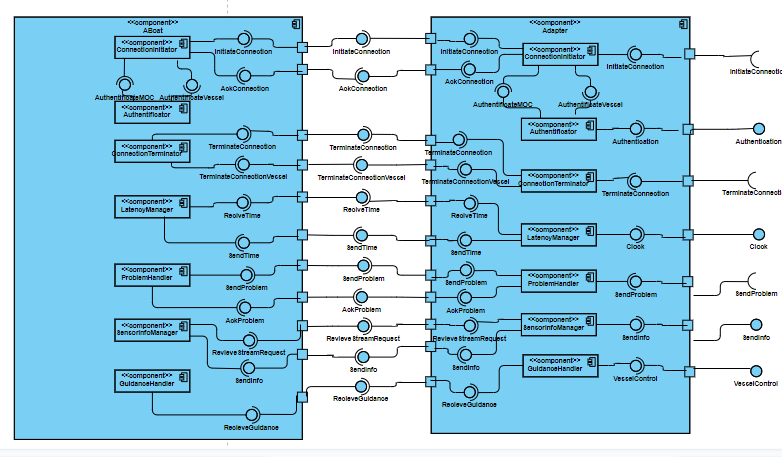
\includegraphics[width=\linewidth]{diagrams/components_adapter}
	\caption{Åboat adapter - VRGP service component diagram}
	\label{fig:adapter-vrgp-component-diagram}
\end{figure}

\end{landscape}

\subsection{Dynamic Design}\label{sec:dynamic-design}

\subsubsection{Activity Diagram}

This high-level activity diagram (figure \ref{fig:activity-diagram}) provides an overview of the general communication flow in the VRGP protocol, including the connection establishment and authentication, the messages that can be sent continuously while the connection is up and the termination of the connection.

\begin{figure}[ht]
	\centering
	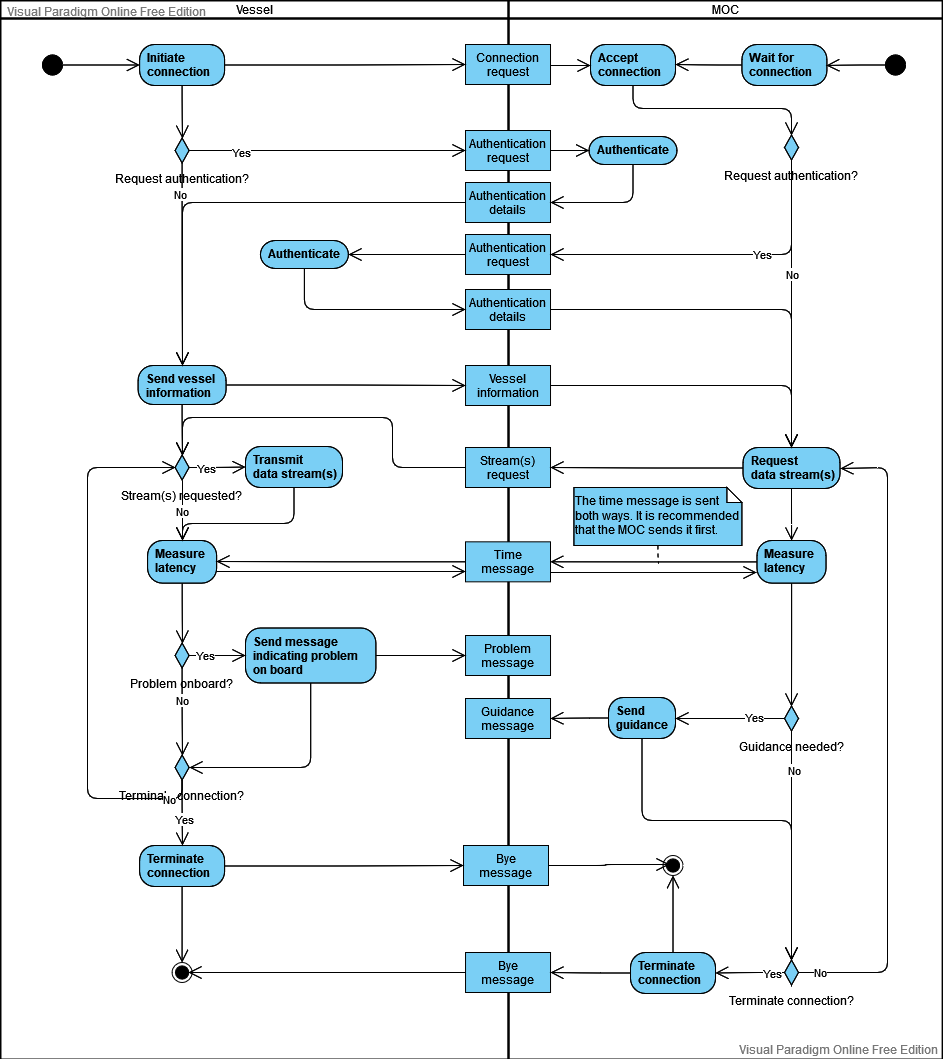
\includegraphics[width=\linewidth]{diagrams/activity-diagram}
	\caption{Activity diagram}
	\label{fig:activity-diagram}
\end{figure}

\subsection{User Interface Design}\label{sec:ui-design}

\subsubsection{Vessel List View}

A MOC can manage arbitrarily many vessel connections at the same time. Therefore, the starting view of the MOC frontend displays a list of all connected vessels including the name, the current latency and the MMSI of the vessel (see \ref{fig:gui-overview}). For each vessel, a detailed view can be accessed by clicking the respective row of the table.

\begin{figure}[ht]
	\centering
	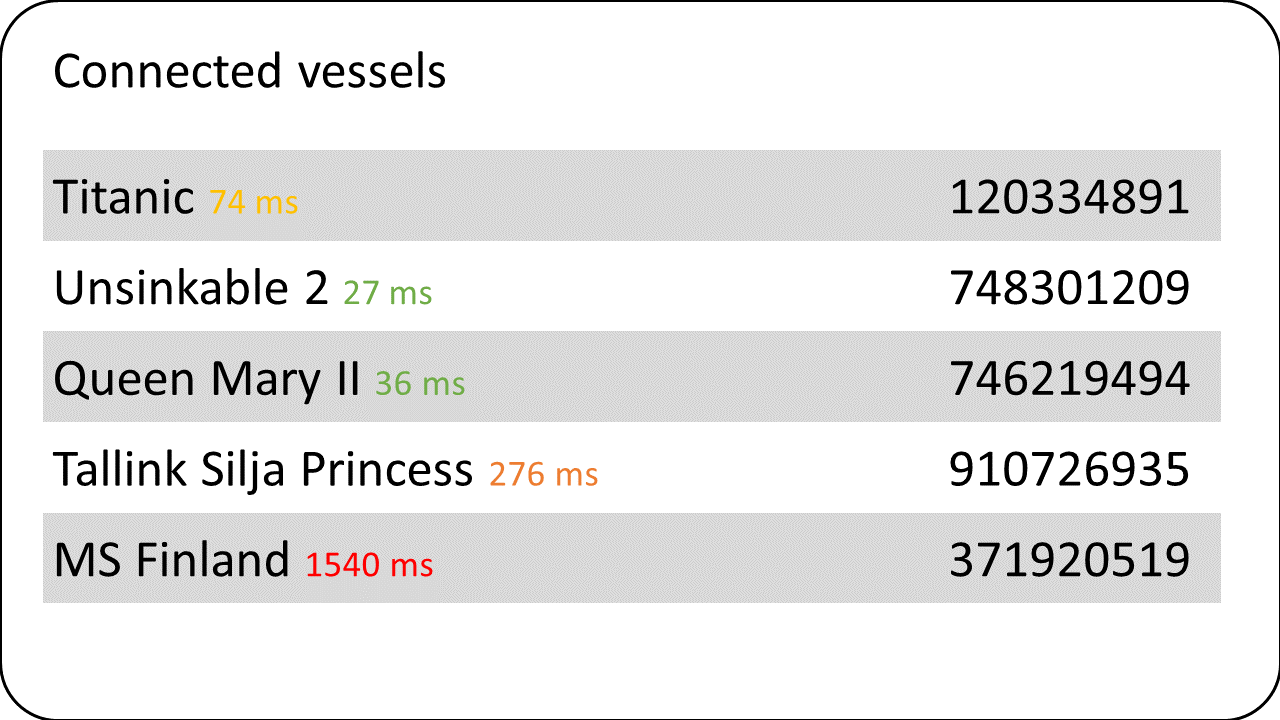
\includegraphics[width=\linewidth]{images/gui-overview}
	\caption{Vessel list view}
	\label{fig:gui-overview}
\end{figure}

\subsubsection{Single Vessel View}

The detailed view for each vessel contains all static and dynamic information of that vessel as well as several possible interactions (see \ref{fig:gui-vessel}).
The view is split into static vessel information at the top of the page and dynamic information as well as possible interactions in the bottom. The "Terminate" button is placed in the top right corner as is standard for closing buttons.
The "Vessel information" tile is placed at the top of the page to make it easily available when entering the detail view.
In the "Information streams" tile, the sensor data as well as the corresponding "Request" buttons are grouped to have all dynamic information in one place. To the right, it is possible to directly react to events on the vessel by typing and sending a guidance message.
At the top left of the page, the name of the vessel is displayed and in the top right, there is a button to terminate the connection between the MOC and the vessel.

\begin{figure}[ht]
\centering
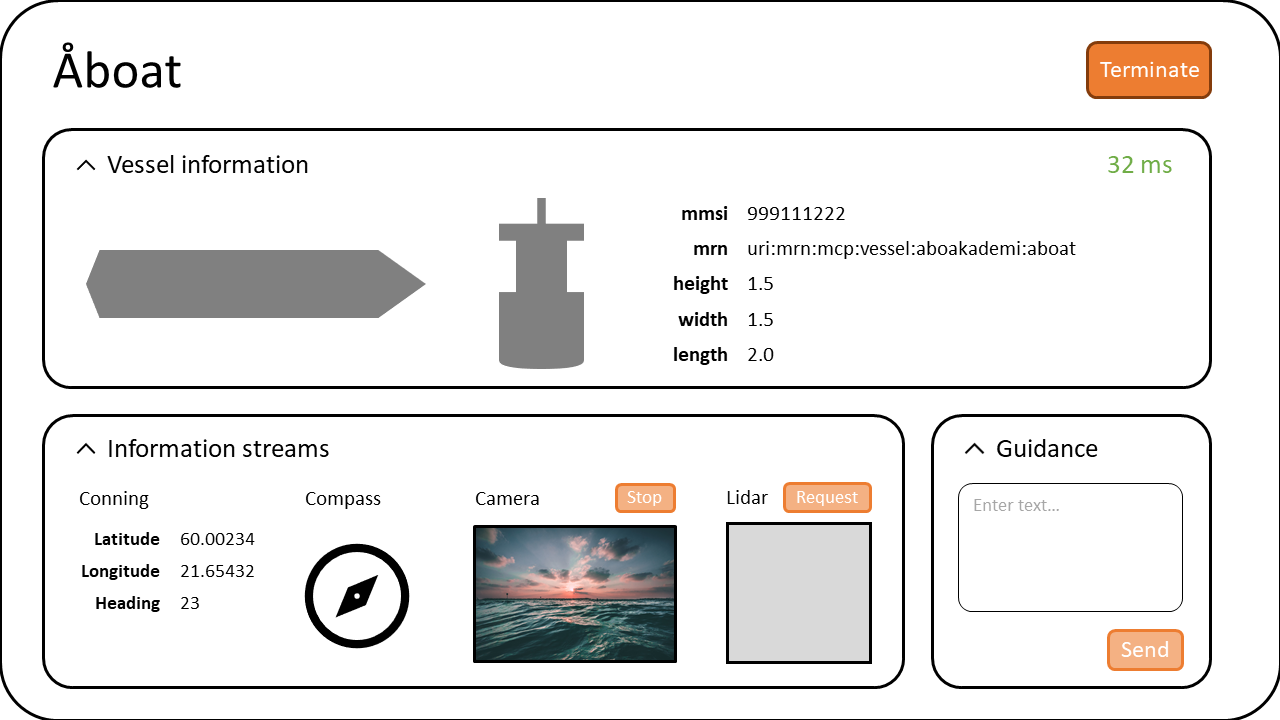
\includegraphics[width=\linewidth]{images/gui-vessel}
\caption{Single vessel view}
\label{fig:gui-vessel}
\end{figure}
